\scanpage{34}
\[
\begin{aligned}
\varphi(a_i,a_{i+1})&=-\beta_0\cdots\beta_i\\
f(a_i)&=\deleted{\unsure{b|\beta}}\beta_0\cdots\beta_{i-1}&
\frac{\varphi(a_i,a_{i+1})^2}{f(a_i)\,f(a_{i+1})}&=\beta_i\,[=4\cos^2\theta_i]\\
f(a_{i+1})&=\beta_0\cdots\beta_i
\end{aligned}
\]
\[
\bigl[\alpha_i=\beta_i-2=2\bigl[\underbrace{2\cos^2\theta_i-1}_{\cos2\theta_i}\bigr]=2\cos2\theta_i\bigr]
\]
$\alpha_i$ est l'\uline{invariant de} $\tau_{a_i}\tau_{\unsure{a_{i+1}|i+1}}$ (rotation)

\figure{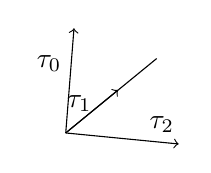
\begin{tikzpicture}[scale=.7]
\draw[->] (0,0)--(.15,1.9) node[left,pos=.66] {$\tau_0$};
\draw (0,0)--(1.65,1.35);
\draw[->] (0,0)--(.95,.78) node[left,pos=.68] {$\tau_1$};
\draw[->] (0,0)--(2.05,-.20) node[above,pos=.85] {$\tau_2$};
\end{tikzpicture}}
$\alpha_0,\alpha_1$
\[
\underbrace{\tau_0\ \tau_1}\ \tau_2\llap{$\underbrace{\phantom{\tau_1\ \tau_2}}$}
\qquad
\rho_0=\tau_0\tau_1\quad \rho_1=\tau_1\tau_2
\]
\figure{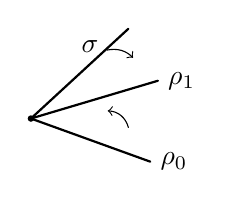
\begin{tikzpicture}[scale=.75,line cap=round]
\fill (0,0) circle (.055);
\draw[thick] (0,0)--(1.65,1.52) node[left,pos=.8] {$\sigma$};
\draw[thick] (0,0)--(2.15,.64) node[right] {$\rho_1$};
\draw[thick] (0,0)--(2.02,-.73) node[right] {$\rho_0$};
\draw[->] (1.29,1.16) to[bend left=27] (1.73,1.03);
\draw[->] (1.65,-.15) to[bend right=36] (1.30,.13);
\end{tikzpicture}}
\[
\tau_0=\rho_0\tau_1\qquad \tau_2=\tau_1\rho_1\qquad
\tau_0\tau_2=\rho_0\rho_1=\sigma\qquad \sigma^2=1\quad \text{i.e. }\tau_0,\tau_2\ \text{comm.}
\]
\[
\tau_0^2=\rho_0\tau_1\rho_0\tau_1=\rho_0\rho_0^{-1}=\mathrm{id}
\]

?? \uline{Prop} Soit
\[
\begin{aligned}
G_2&=(\underline{\tau}_0,\underline{\tau}_1,\underline{\tau}_2\mid
\underline{\tau}_0^2=\underline{\tau}_1^2=\underline{\tau}_2^2=(\underline{\tau}_0\underline{\tau}_2)^2=1)\\
\rotatebox{90}{$\hookrightarrow$}\quad &\\[-1ex]
G_2^+&=(\underline{\rho}_0,\underline{\rho}_1\mid(\underline{\rho}_0\underline{\rho}_{\unsure{+|1}})^2=1)
\end{aligned}
\]
\diagram{\begin{tikzcd}[ampersand replacement=\&,column sep=small]
\tau_0\tau_1 \& \tau_1\tau_2\\
\rho_0\arrow[u] \&\rho_1\arrow[u,dash]
\end{tikzcd}}

Considérons fibré projectif \inserted{$X$} sur $S$, \inserted{\deleted{\unsure{X}} de rg $N\geq1$} et \deleted{\unsure{catégorie|catégories}}, $G=\mathrm{Aut}(X)$. \deleted{Alors \illegible{1} Alors} Soit $\mathrm{Hom}^!(G_2,G)$ le sous-ensemble des $\mathrm{Hom}_{\mathrm{gr}}(G_2,G)$ formé des $\varphi$ telles que $\tau_i\overset{\mathrm{dfn}}{=}\varphi(\underline{\tau}_i)$ \unsure{soit|soient} une \uline{réflexion} $(i=0,1,2)$, et que $(\tau_0,\tau_1)\ (\tau_1,\tau_2)$ et $(\underbrace{\tau_0\tau_1}_{\unsure{\rho|{}}}\overset{\mathrm{dfn}}{=}\rho_0,\enspace \tau_1\tau_2\overset{\mathrm{dfn}}{=}\rho_{\unsure{2|1}})$ ne commutent pas \inserted{fibre par fibre} (i.e. $\rho_0^2\ne\mathrm{id}$, $\rho_1^{\unsure{2|{}}}\ne\mathrm{id}$, $\rho_0\rho_1\ne\rho_1\rho_0$ fibre \unsure{p|par} fibre.

% archive sheet number: 33
% slanted
\margin{\uline{NB} $\rho_0$ et $\rho_1$ ne \unsure{comm.} pas \unsure{entre eux} $\Longleftrightarrow$ $\tau_1$ et $\sigma$ ne commutent pas $\Longleftrightarrow$ $\sigma$ \unsure{fixe|permute} \unsure{autr.} les \illegible{1} \unsure{conditions|d'autres} \unsure{j'}\illegible{1} on \unsure{estime} que $\tau_0,\tau_2$ et $\sigma$ \unsure{ne soient permut.} pour cette \unsure{hypothèse}.}

Soit $\mathrm{Hom}^!(G_{\unsure{2|4}}^+,G)$ le sous-ensemble de $\mathrm{Hom}_{\mathrm{gr}}(G_2^+,G)$ formé des $\varphi^+$ telles que $[\deleted{\unsure{\rho=\varphi^+(\rho)}}\ \rho_0=\varphi^+(\underline{\rho}_0),\rho_1=\varphi^+(\underline{\rho}_1)]$ on ait : $\rho_0^2\ne1$, $\rho_1^{\unsure{2|{}}}\ne1$, $\rho_0\rho_1\ne\rho_1\rho_0$ sur chaque fibre, et (si $N\geq\deleted{\unsure{1}}2$) $\exists$ loc. sur \unsure{$S$|la base|{}} fibré projectif \inserted{de $Z$ de $X$, de codim $3$, et des} \deleted{tel que \unsure{fibre par fibre} $\rho_0|X_0=\rho_1|X_0=\mathrm{id}_{X_0}$.}
% long insertion from the foot of the sheet
\inserted{projectifs $X_0,X_1,X_2\supset Z$ de codim $2$, \inserted{$X_0\cap X_1\cap X_2=Z$,} tels que $\rho_0,\rho_1,\sigma=\rho_0\rho_1$ induisent l'identité resp. sur $X_0,X_1,X_2$ [si $N=2,3$ il faut \deleted{sans} doit \uline{se donner} les $X_i$, si $N\geq4$ ils sont uniques\ldots]}

\uline{Alors} l'application $\varphi\longmapsto\varphi^+=\varphi\mid G_2^+$ sera bijective. (?)

\margin{TSVP}
